\begin{figure}[htb]
    \begin{center}
    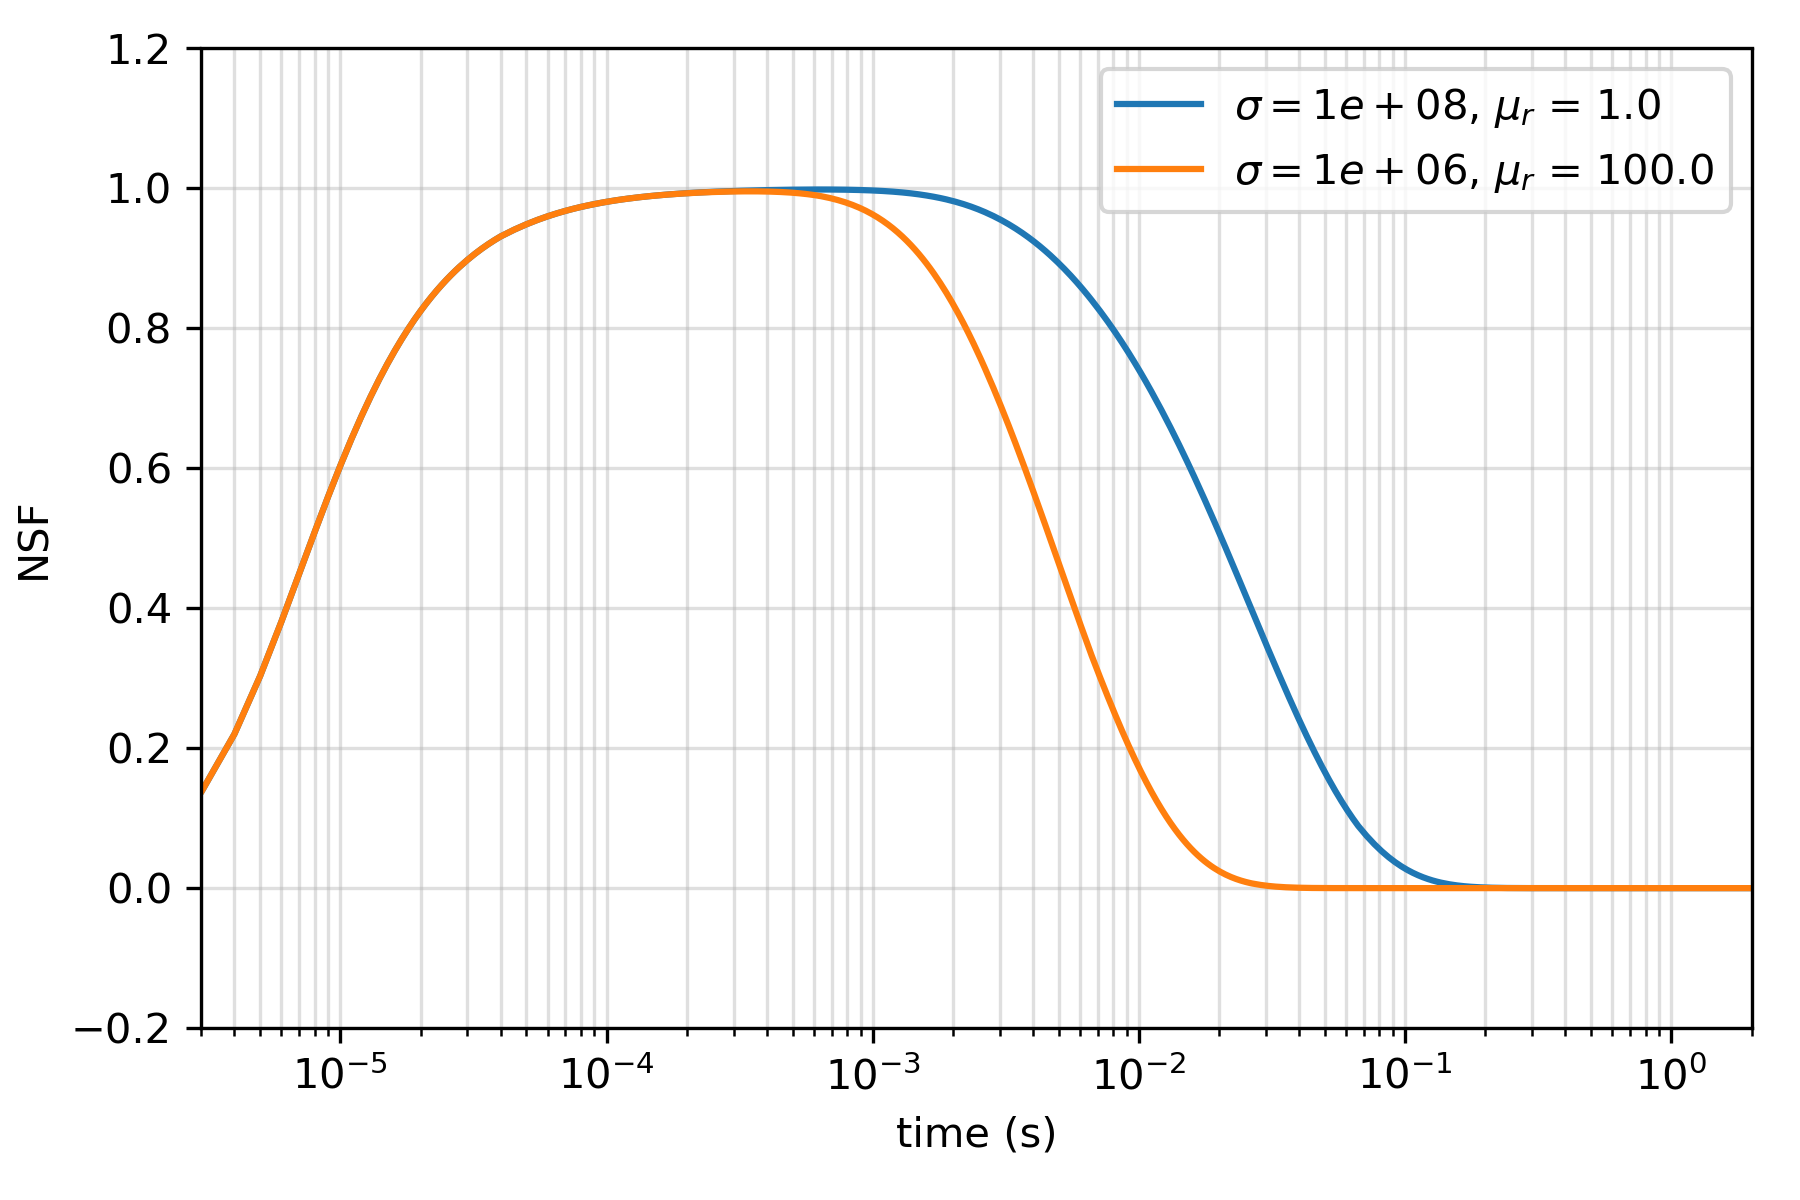
\includegraphics[width=0.6\columnwidth]{figures/casing_software/tdemNSF.png}
    \end{center}
\caption{
    Normalized secondary field (NSF) through time.
    In the time-domain, we compute the NSF by taking the difference between the total magnetic flux at the receiver and the whole-space response
    and then taking the ratio with the whole-space magnetic flux prior to shutting off the transmitter.
}
\label{fig:tdemNSF}
\end{figure}
